\section{Comprensione del dominio e elicitazione dei requisiti}
Rappresenta la prima fase della spirale della figura \ref{fig:cycle-requirements}.
Per acquisire informazioni riguardo i requisiti vengono eseguite certe attività:
\begin{itemize}
	\item studiare il system-as-is:
	\begin{itemize}
		\item organizzazione aziendale: la struttura, le dipendenze, gli obbiettivi strategico, le politiche, i flussi di lavoro, le procedure operazionali;
		\item il dominio di applicazione: i concetti, gli obbiettivi, i compiti, i vincoli, i regolamenti;
		\item analisi di problemi con il system-as-is: le cause, le conseguenze;
	\end{itemize}
	\item analizzare le opportunità tecnologiche, le condizioni di mercato più recenti;
	\item identificare gli \textbf{stakeholders} di sistema;
	\item identificare gli obbiettivi da migliorare, i vincoli organizzativi e tecnologici del system-to-be; le opzioni alternative per soddisfare gli obbiettivi, per assegnare responsabilità; gli scenari di un ipotetica interazione con l'ambiente software, i requisiti sul software, le assunzioni sull'ambiente.
\end{itemize}
\subsection{Tecniche di elicitazione}
Vi sono due tecniche principali di elicitazione:
\begin{enumerate}
	\item \textbf{Artefact-driven}: orientata agli artefatti disponibili
	\item \textbf{Stakeholder-driven}: orientata al coinvolgimento degli stakeholders.
\end{enumerate}
\subsection{Analisi degli stakeholders}
La cooperazione degli stakeholder è essenziale per un RE di successo. Deve essere selezionato un campione rappresentativo per assicurare una copertura adeguata, comprensiva del problema del mondo reale.
La selezione avviene in base alla posizione dell'organizzazione, al ruolo nel prendere le decisioni, il tipo di contributo alla conoscenza che porta, livello di esposizione ai problemi, interessi personali, potenziali conflitti (differenti tipologie di utenti possono avere necessità distinte e anche in conflitto perché magari vogliono guadagnare una qualche forma di posizione di vantaggio all'interno dell'azienda).

Acquisire la conoscenza dagli stakeholder è difficile perché:
\begin{itemize}
	\item sorgenti di informazioni diverse, punti di vista in contrapposizione;
	\item difficoltà ad accedere alle persone chiave (più in alto sono nella gerarchia aziendale, più probabile è la loro indisponibilità perché coprono ruoli critici);
	\item background, terminologia e cultura differenti (che vuol dire che, persone diverse potrebbero utilizzare una terminologia differente);
	\item conoscenza tacita, necessità nascoste: alcuni soggetti potrebbero sottintendere concetti perché sono dati per scontato;
	\item dettagli irrilevanti: l'utente esprime, attraverso esempi, dettagli irrilevanti;
	\item resistenza al cambiamento, politiche interne, competizione: le persone cambiano difficilmente le proprie abitudini (dal ramo operativo, al ramo dirigenziale);
	\item cambio del personale, cambiamenti nell'organizzazione, cambiamenti nelle priorità.
\end{itemize}
L'ingegnere dei requisiti deve avere diverse soft-skills: abilità di comunicazione, capacità di ascolto, stabilire una relazione di fiducia, capacità di riformulare le conoscenze e di ristrutturarle in continuazione.

\subsubsection{Background study} Serve per capire il dominio in cui l'azienda opera. Consiste nel raccogliere conoscenza di base a partire da informazioni provenienti dall'organizzazione aziendale che si sta studiando. I documenti devono contenere informazioni riguardo:
\begin{itemize}
	\item l'\textbf{organizzazione:} avviene attraverso la consultazione di grafici organizzativi (ad esempio un albero in cui vengono rappresentati i ruoli dei dipendenti), piani di business (quali sono le strategie messe in atto dall'azienda per raggiungere gli obbiettivi), report finanziari, verbali delle riunioni (cosa è stato detto durante le riunioni);
	\item \textbf{dominio:} attraverso libri, articoli, sondaggi, regolamentazioni, report su sistemi simili che operano nello stesso dominio;
	\item \textbf{system-as-is:} consultando la documentazione delle procedure aziendali, regole di business, documenti scambiati, le richieste di cambiamento, i report che contengono dei difetti riscontrati, delle lamentele degli utenti (in alcuni ambiti, è obbligatorio per legge);
\end{itemize}
L'ingegnere dei requisiti utilizza lo studio di background per comunicare più efficacemente con gli stakeholders.

L'attività di raccolta dei requisiti potrebbe essere onerosa in termini di tempo, perché il materiale da analizzare durante il background study potrebbe essere datato, contenere dettagli irrilevanti. Una possibile soluzione è data dall'utilizzo di metadati per filtrare la documentazione (intesa come fonte di informazioni provenienti dall'organizzazione aziendale).

\subsubsection{Data collection}
Consiste nella raccolta di dati, fatti aziendali, quindi informazioni quantitative. Questo tipo di valutazioni serve per ottenere requisiti \textbf{non funzionali}. Un problema nell'elicitazione dei requisiti. è ottenere dati affidabili e riuscire ad interpretarli correttamente.
\subsubsection{Questionari} Consiste nel somministrare agli stakeholders, una lista di domande (aperte o chiuse) per raccogliere informazioni che riguardano il system-as-is. Le domande possono essere a crocette, a risposta multipla, espresse in una scala ordinale. Questa tecnica è efficace per raccogliere informazioni velocemente e in maniera economica, senza la necessità di recarsi presso gli stakeholders.

La formulazione delle domande all'interno dei questionari richiede di prestare molta attenzione,   in particolare a non suggerire le risposte agli stakeholders o inserire un bias nelle domande. Ogni domanda deve essere chiara, non ambigua. Ci sono delle linee guida che possono essere seguite per formulare correttamente i questionari. È importante fare un \textbf{cross-check}, riformulando più volte la stessa domanda per assicurare la non presenza di inconsistenze nelle risposte.
I questionari potrebbero essere controllati da terze parti per verificare la consistenza delle risposte.
\subsubsection{Card sort} L'obbiettivo del \textbf{card sort} è di acquisire ulteriore informazione rispetto ai concetti estratti con i questionari. Le informazioni raccolte riguardanti il system-as-is e le funzionalità del software vengono scritte in delle carte che gli utenti devono successivamente raggruppare. L'obbiettivo è di cogliere i ragionamenti fatti dagli utenti su come hanno raggruppato le carte e perché. Tipicamente in questa fase emergono nuovi requisiti riguardanti i legami fra gli oggetti delle carte. Ad esempio, si consideri un'applicazione di pianificazione dei web meeting. Nella prima iterazione, un gruppo di utenti potrebbe collegare la carta "meeting" a quella "partecipanti". Nasce il requisito di \textit{invito di un partecipante}. Nella seconda iterazione, un altro gruppo potrebbe creare la stessa relazione tra le stesse carte meeting e partecipante dando una motivazione diversa, ad esempio \textit{i vincoli di agenda dei vari partecipanti devono essere noti al sistema per poterli salvare in maniera autonoma}.
\subsubsection{Repertory grid} Una griglia come quella in figura \ref{fig:repertorygrid} è detta \textbf{repertory grid} che raccoglie una relazione tra una lista di concetti e una lista di attributi. Gli utenti forniscono per ciascuna coppia un valore definito fra quelli disponibili nella griglia. Il \textbf{conceptual laddering} è l'attività successiva al repertory grid, in cui viene chiesto all'utente di raggruppare i concetti simili della griglia, fornire un nome per ciascuno di essi.
\begin{figure}[th]
	\centering
	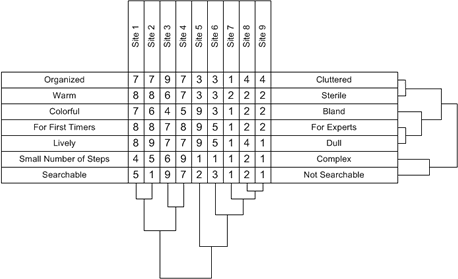
\includegraphics[width=0.7\linewidth]{img/repertory_grid}
	\caption{esempio di repertory grid.}
	\label{fig:repertorygrid}
\end{figure}
Questa tecnica è abbastanza semplice da realizzare, facile ed economica ma i risultati potrebbero essere soggettivi, irrilevanti o imprecisi.
\subsubsection{Scenari e storyboard}

